\section{STP}
\subsection{STP의 개념}
    Spanning Tree Protocol (STP)는 브리지/스위치로 연결된 네트워크에서 Switching loop를 발견, 방지, 제거하는 protocol이다.  STP는 Spanning Tree 형태의 topology를 만드는 알고리즘에서 기초하여 Loop내의  특정한 포트를 차단시켜 그 Link로 Frame을 전달하지 않아, Loop로부터 자유로운 Redundant Topology를 제공한다. 연결된 Link에 문제가 생기면 차단된 Link를 다시 활용하여 Spanning Tree를 구성할 수 있다. \\
    \vspace{-4mm}
    \begin{figure}[!h]\centering
		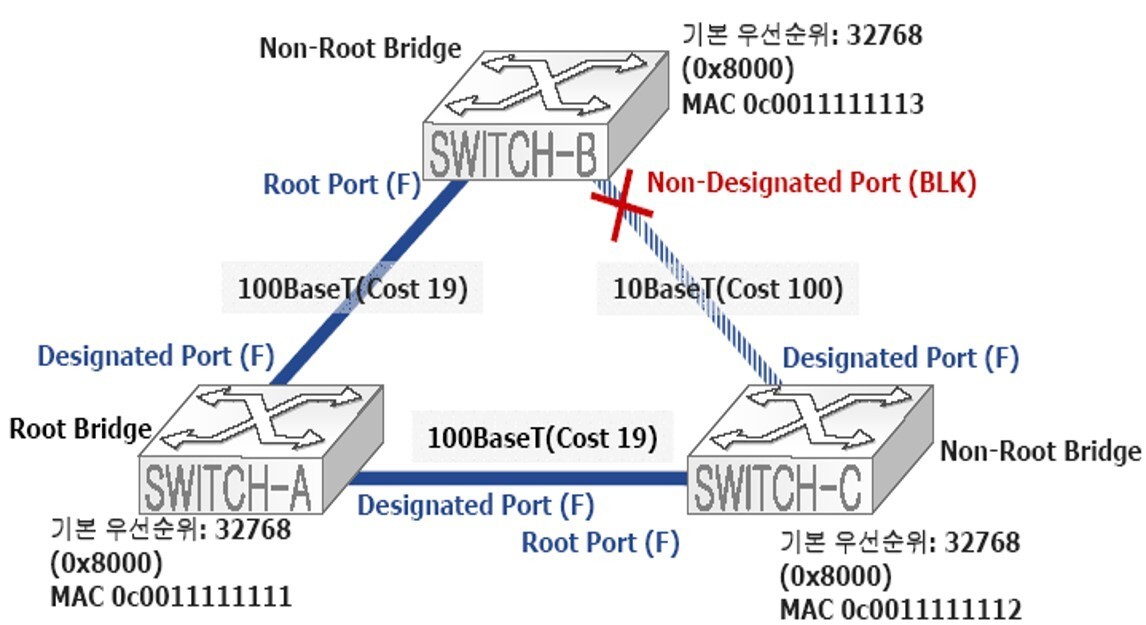
\includegraphics[width=.65\textwidth]{image/week06/2-1.png}
		\caption{\small Spanning Tree Protocol}
		\vspace{-10pt}
    \end{figure}
    
\subsection{STP의 동작}
    \subsubsection*{BDPU 교환}
    모든 스위치는 2초 간격으로 BDPU (Bridge Protocol Data Unit)라는 특수 목적의 Frame을 통해 Spanning Tree 관련 정보를 송수신한다. BDPU에는 브리지 ID, 경로, 포트 정보 등의 정보가 담겨있고, 이 정보를 통해 스위치 선출 및 Switching Loop 차단을 하게된다. \\
    \subsubsection*{Switching Loop 차단}
    각 스위치에서 루트 스위치로 가는 각 경로의 경로 비용을 계산하여 경로 비용이 가장 낮은 경로만 유지하고, 다른 경로는 중단시킨다. 주로 루핑 포트 중 하나를 차단시키는 방식으로 운용된다. \\
    
\subsection{STP 선출 및 차단 과정}
    \begin{enumerate}
        \item 루트 스위치 선출 : 가장 낮은 BID 값 (브리지 우선순위 + MAC 주소)을 갖는 스위치를 루트 스위치로 선출
        \item 루트 포트 결정 : 루트 스위치까지의 최단경로비용을 계산하여, Non-Root 스위치 마다 하나의 루트 포트를 결정.
        \item 지정 포트 결정 : Segment당 하나의 지정 (Designated) 포트를 결정
        \item 비지정 포트 봉쇄 : 루트 포트도, 지정 포트도 아닌 포트를 비지정 포트로 결정하여 최종적으로 차단
    \end{enumerate}
\newpage